% This is "sig-alternate.tex" V2.0 May 2012
% This file should be compiled with V2.5 of "sig-alternate.cls" May 2012
%
% This example file demonstrates the use of the 'sig-alternate.cls'
% V2.5 LaTeX2e document class file. It is for those submitting
% articles tol ACM Conference Proceedings WHO DO NOT WISH TO
% STRICTLY ADHERE TO THE SIGS (PUBS-BOARD-ENDORSED) STYLE.
% The 'sig-alternate.cls' file will produce a similar-looking,
% albeit, 'tighter' paper resulting in, invariably, fewer pages.
%
% ----------------------------------------------------------------------------------------------------------------
% This .tex file (and associated .cls V2.5) produces:
%       1) The Permission Statement
%       2) The Conference (location) Info information
%       3) The Copyright Linle with ACM data
%       4) NO page numbers
%
% as against the acm_proc_article-sp.cls file which
% DOES NOT produce 1) thru' 3) above.
%
% Using 'sig-alternate.cls' you have control, however, from within
% the source .tex file, over both the CopyrightYear
% (defaulted to 200X) and the ACM Copyright Data
% (defaulted to X-XXXXX-XX-X/XX/XX).
% e.g.
% \CopyrightYear{2007} will cause 2007 to appear in the copyright line.
% \crdata{0-12345-67-8/90/12} will cause 0-12345-67-8/90/12 to appear in the copyright line.
%
% ---------------------------------------------------------------------------------------------------------------
% This .tex source is an example which *does* use
% the .bib file (from which the .bbl file % is produced).
% REMEMBER HOWEVER: After having produced the .bbl file,
% and prior to final submission, you *NEED* to 'insert'
% your .bbl file into your source .tex file so as to provide
% ONE 'self-contained' source file.
%
% ================= IF YOU HAVE QUESTIONS =======================
% Questions regarding the SIGS styles, SIGS policies and
% procedures, Conferences etc. should be sent to
% Adrienne Griscti (griscti@acm.org)
%
% Technical questions _only_ to
% Gerald Murray (murray@hq.acm.org)
% ===============================================================
%
% For tracking purposes - this is V2.0 - May 2012

\documentclass{sig-alternate-2013}

\usepackage{subfigure}
\usepackage{epsfig}
\usepackage[ruled]{algorithm2e}
\usepackage{algorithmic}

\newfont{\mycrnotice}{ptmr8t at 7pt}
\newfont{\myconfname}{ptmri8t at 7pt}
\let\crnotice\mycrnotice%
\let\confname\myconfname%

\permission{Permission to make digital or hard copies of all or part of this work for personal or classroom use is granted without fee provided that copies are not made or distributed for profit or commercial advantage and that copies bear this notice and the full citation on the first page. Copyrights for components of this work owned by others than ACM must be honored. Abstracting with credit is permitted. To copy otherwise, or republish, to post on servers or to redistribute to lists, requires prior specific permission and/or a fee. Request permissions from permissions@acm.org.}
\conferenceinfo{MM'14,}{November 03 - 07 2014, Orlando, FL, USA.}
\copyrightetc{Copyright 2014 ACM \the\acmcopyr}
\crdata{978-1-4503-3063-3/14/11\ ...\$15.00.\\
http://dx.doi.org/10.1145/2647868.2654905}

\clubpenalty=10000
\widowpenalty = 10000

\begin{document}
%
% --- Author Metadata here ---
%\conferenceinfo{WOODSTOCK}{'97 El Paso, Texas USA}
%\CopyrightYear{2007} % Allows default copyright year (20XX) to be over-ridden - IF NEED BE.
%\crdata{0-12345-67-8/90/01}  % Allows default copyright data (0-89791-88-6/97/05) to be over-ridden - IF NEED BE.
% --- End of Author Metadata ---

\title{Social Embedding Image Distance Learning}

%
% You need the command \numberofauthors to handle the 'placement
% and alignment' of the authors beneath the title.
%
% For aesthetic reasons, we recommend 'three authors at a time'
% i.e. three 'name/affiliation blocks' be placed beneath the title.
%
% NOTE: You are NOT restricted in how many 'rows' of
% "name/affiliations" may appear. We just ask that you restrict
% the number of 'columns' to three.
%
% Because of the available 'opening page real-estate'
% we ask you to refrain from putting more than six authors
% (two rows with three columns) beneath the article title.
% More than six makes the first-page appear very cluttered indeed.
%
% Use the \alignauthor commands to handle the names
% and affiliations for an 'aesthetic maximum' of six authors.
% Add names, affiliations, addresses for
% the seventh etc. author(s) as the argument for the
% \additionalauthors command.
% These 'additional authors' will be output/set for you
% without further effort on your part as the last section in
% the body of your article BEFORE References or any Appendices.
\numberofauthors{1} %  in this sample file, there are a *total*
% of EIGHT authors. SIX appear on the 'first-page' (for formatting
% reasons) and the remaining two appear in the \additionalauthors section.
%
\author{
% You can go ahead and credit any number of authors here,
% e.g. one 'row of three' or two rows (consisting of one row of three
% and a second row of one, two or three).
%
% The command \alignauthor (no curly braces needed) should
% precede each author name, affiliation/snail-mail address and
% e-mail address. Additionally, tag each line of
% affiliation/address with \affaddr, and tag the
% e-mail address with \email.
%
% 1st. author
\alignauthor
Shaowei Liu${}^1$, Peng Cui${}^1$, Wenwu Zhu${}^1$, Shiqiang Yang${}^1$ and Qi Tian${}^2$\\
\affaddr{${}^1$Computer Science Department, Tsinghua University, China}\\
\affaddr{${}^1$Tsinghua National Laboratory for Information Science and Technology}\\
\affaddr{${}^2$Department of Computer Science, University of Texas at San Antonio}\\
\small{\email{liu-sw11@mails.tsinghua.edu.cn, cuip/wwzhu/yangshq@tsinghua.edu.cn,  qitian@cs.utsa.edu}}
% 2nd. author
%\alignauthor
%G.K.M. Tobin\titlenote{The secretary disavows
%any knowledge of this author's actions.}\\
%       \affaddr{Institute for Clarity in Documentation}\\
%       \affaddr{P.O. Box 1212}\\
%       \affaddr{Dublin, Ohio 43017-6221}\\
%       \email{webmaster@marysville-ohio.com}
%% 3rd. author
%\alignauthor Lars Th{\o}rv{\"a}ld\titlenote{This author is the
%one who did all the really hard work.}\\
%       \affaddr{The Th{\o}rv{\"a}ld Group}\\
%       \affaddr{1 Th{\o}rv{\"a}ld Circle}\\
%       \affaddr{Hekla, Iceland}\\
%       \email{larst@affiliation.org}
%\and  % use '\and' if you need 'another row' of author names
%% 4th. author
%\alignauthor Lawrence P. Leipuner\\
%       \affaddr{Brookhaven Laboratories}\\
%       \affaddr{Brookhaven National Lab}\\
%       \affaddr{P.O. Box 5000}\\
%       \email{lleipuner@researchlabs.org}
%% 5th. author
%\alignauthor Sean Fogarty\\
%       \affaddr{NASA Ames Research Center}\\
%       \affaddr{Moffett Field}\\
%       \affaddr{California 94035}\\
%       \email{fogartys@amesres.org}
%% 6th. author
%\alignauthor Charles Palmer\\
%       \affaddr{Palmer Research Laboratories}\\
%       \affaddr{8600 Datapoint Drive}\\
%       \affaddr{San Antonio, Texas 78229}\\
%       \email{cpalmer@prl.com}
}
% There's nothing stopping you putting the seventh, eighth, etc.
% author on the opening page (as the 'third row') but we ask,
% for aesthetic reasons that you place these 'additional authors'
% in the \additional authors block, viz.
%\additionalauthors{Additional authors: John Smith (The Th{\o}rv{\"a}ld Group,
%email: {\texttt{jsmith@affiliation.org}}) and Julius P.~Kumquat
%(The Kumquat Consortium, email: {\texttt{jpkumquat@consortium.net}}).}
% Just remember to make sure that the TOTAL number of authors
% is the number that will appear on the first page PLUS the
% number that will appear in the \additionalauthors section.

\maketitle

\begin{abstract}
Image distance (similarity) is a fundamental and important problem in image processing. However, traditional visual features based image distance metrics usually fail to capture human cognition. This paper presents a novel Social embedding Image Distance Learning (\emph{SIDL}) approach to embed the similarity of collective social and behavioral information into visual space. The social similarity is estimated according to multiple social factors. Then a metric learning method is especially designed to learn the distance of visual features from the estimated social similarity. In this manner, we can evaluate the cognitive image distance based on the visual content of images. Comprehensive experiments are designed to investigate the effectiveness of \emph{SIDL}, as well as the performance in the image recommendation and reranking tasks. The experimental results show that the proposed approach makes a marked improvement compared to the state-of-the-art image distance metrics. An interesting observation is given to show that the learned image distance can better reflect human cognition.
\end{abstract}


% A category with the (minimum) three r equired fields
\category{H.3.3}{Information Search and Retrieval}{Retrieval models}

\terms{Algorithms, Experimentation, Performance}

\keywords{image search and recommendation, social similarity, user behavior, metric learning}

\vspace{-0.3cm}\section{INTRODUCTION}
With the fast development of Internet, images play an important role in delivering information in our daily life. Thus, understanding images become an increasing demand. In image processing and understanding applications, such as image search, recommendation and classification, measuring the distance (or similarity) of pair-wise images is a fundamental and important issue. \emph{If an effective image distance metric is obtained, we can easily employ existing technologies to achieve satisfactory performance in such applications\cite{visualrank,cbf}.}

However, to date, existing image distance metrics do not perform well to achieve this goal, due to the fact that they usually focus on measuring similarity of visual features but are not mature to capture user intention, especially in human related applications, such as image search and recommendation. Here user intention includes many aspects, such as semantics, attributes, emotion, layout, etc. Although the problem of capturing user intention has received increasing attention, how to identify and understand it is still a great challenge because there is a huge gap between level visual contents and high level user intention, which is called intention gap.

 With the development of social network, a huge amount of users share their beautiful pictures and view others' in the social media platforms, such as Flickr and Twitter. Within these platforms, we can obtain not only vast amounts of images but also a series of collective social and behavioral information, such as annotated tags, favorite images and interest groups of users. In social psychology, it has been proved that human cognition and user behavior influence each other \cite{cognitive}. Therefore, social behavioral information in social media platform can be regarded as the reflection of their intention when viewing images. Given user behavior information in the social media platforms, we can use to better evaluate image distance. In recent years, there are some works that focus on using social information to better evaluate image similarity and achieves some improvements. However, they are limited due to the following challenges:


 %Although the technologies up to date can hardly estimate the user cognition behind his behavior, we can easily evaluate the similarity of user behaviors of two images. For a pair of images, if users have similar behaviors (such as favoring, sharing and tagging), their cognition to the images would also be similar. In this paper, we refer to the similarity of users' social behaviors as social similarity.



(1) \textbf{The lack of social information in general Web image.} Although behavioral information does help to estimate user cognition, most of the Web images do not have user behavior information due to the fact that they are not produced by social media platforms. If the image distance relies on  social behavioral data, our method will be extremely circumscribed in social images. Therefore, how to make our distance metric universal in common Web images is a great challenge in our problem.

(2) \textbf{The unreliability and sparsity of social media data.} In social network, collective social and behavioral information is usually sparse and unreliable. If the amount of user behavior information is not enough, the social similarity may have contingency. Not all of image pairs's social similarity can be evaluated well. Thus, we also need to consider the reliability of social similarity and balance the social similarity and visual similarity in this case.

(3) \textbf{The sparsity of user behavior.} 


%(3) The Heterogeneity of social data. Different with traditional homogeneous data structure, the data in social media is heterogeneous  and hybrid. For example, a user may publish and favor a lot of images and an image may be shared to a series of interest groups. Therefore, to make our method extensible, we should formulate these multi-modal information in a unified structure.

\begin{figure*}
\centering
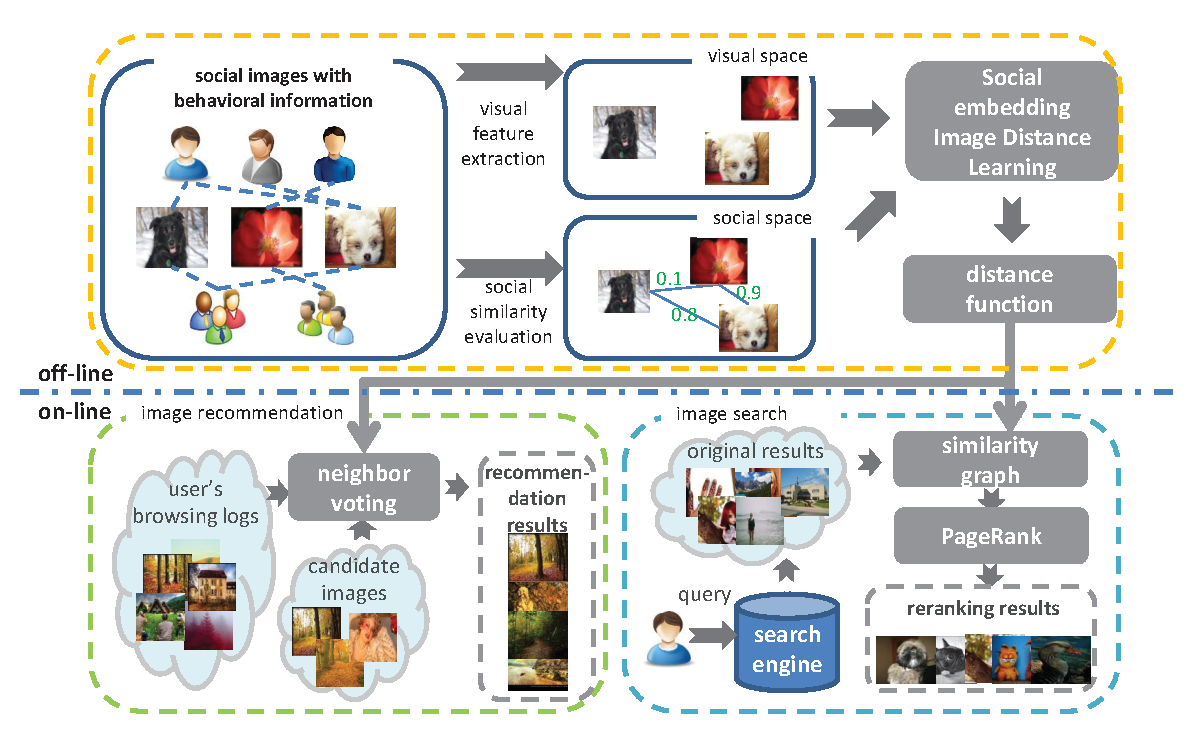
\epsfig{file=framework.eps, width = 5.2in, height = 2.4in}
\caption{Illustration of the proposed Social embedding Image Distance Learning (\emph{SIDL}) approach and the image search and recommendation system developed on \emph{SIDL}.}
\label{framework}
\end{figure*}

To address the above problems, we propose a Social embedding Image Distance Learning (\emph{SIDL}) approach to learn image distance from user behavior information in social media platforms, which is shown in Figure \ref{framework}. In the approach, we use metric learning technique to learn an image distance function of visual features. Different from traditional metric learning work, our distance function aims at making image distance consistent to their social distance in user behavior. Thus, although the distance function is learned from social images (i.e., the images in social media platforms), it can measure the distance of ordinary Web images because it learns the weight and correlation of visual features. We call this idea ``learn from social image, work beyond social image". In our method, we first estimate the social similarity among social images, where the reliability of social entities is evaluated. Next, we conduct our metric learning method to reduce the distance of socially similar images and enlarge the distance of socially dissimilar images. Finally, the learned image distance function is used to evaluate the distance of Web images based on their visual features. The image distance can be applied to a lot of applications, such as image recommendation and reranking. We not only conduct comprehensive experiments to show the effectiveness of our approach, but also give an interesting observation about the relationship between the learned distance and our intuitive cognition.

The contributions of our proposed approach are summarized as follows:

(1) We propose a novel image distance learning approach, which aims at using user behavior information in social media to capture human cognition in Web image distance measuring. To the best of our knowledge, we are the first who use the idea of ``learn from social media, work beyond social media" to solve this problem.

(2) In this paper, we propose a Social Embedding Image Distance Learning approach, where an image distance metric function based on visual features is learned to make image distance consistent to social distance defined from user behavior. In our approach, social distance is well estimated in multimodal social factors. The metric learning method is especially designed to learn the similarity of visual features from social distance. Furthermore, we design two basic application scenarios based on the proposed \emph{SIDL} method, including image recommendation and image reranking.

(3) To evaluate the performance of our approach, comprehensive experiments are conducted based on real social media and image reranking datasets. The experimental results have shown the effectiveness of the learning method. In addition, compared to the state-of-the-art image distance metrics the superiority of our image distance metric in the applications of image recommendation and reranking is also demonstrated.

(4) More than quantitative evaluation, an interesting observation of the relationship between the learned distance and our intuitive cognition is also given to show our results subjectively. We can observe that the key points of images, such as eyes, salient objects, are more important in measuring image similarity.

The rest of the paper is organized as follows: Section 2 gives a brief overview and comparison of related work. Section 3 introduces the evaluation of image social similarity. In Section 4, we introduce optimization of the proposed \emph{SIDL} method and present two applications including image reranking and recommendation based on our distance learning method. Then, we introduce our experiments and report the results in Section 5. Finally, Section 6 summarizes the paper.

\vspace{-0.4cm}\section{RELATED WORK}
Aiming at improving the performance of image search, a series of methods have been proposed to capture human cognition , including query log based methods \cite{click1,  click_bing}, query analysis based methods \cite{query_ana1,mingdong}, relevance feedback based methods \cite{rf, attribute_feedback}, etc. In query log based methods, user click data in image search engines are used to estimate user intention. However, if a query contains less training images, the performance will not be very good. Besides, the image with low rank will not be easily seen by others. Query analysis based methods usually use the techniques in IR, such as query suggestion to capture different aspects of user intention. Zha \emph{et al.} proposed a visual query suggestion approach \cite{visual_suggestion} to suggest more detailed queries for ambiguous queries. In these methods, an important assumption is that visually similar images should have similar user intentions, which is not always tenable. Relevance feedback is another effective way to collect the cognition information by collecting users' feedback. However, the complex operation of feedback may sometimes reduce the user experience.

With the development of social media, a series of social-sensed image search and recommendation approaches have been proposed\cite{cui2014}. The social factors, such as image tags, users, interest groups are considered to replace the original manually labeled data. Image tagging methods \cite{tag1} by user annotation show their significant improvements in bridging the semantic gap. Liu \emph{et al.} proposed an image reranking method \cite{social_visual} that considers both visual factor\cite{zheng2013visual,zhiwang} and social factor. In this work, interest group in Flickr is utilized to evaluate the image similarity in user intention level. The research indicates that the interest groups can help understanding user intention in image reranking. However, this work is based on the images in Flickr, which cannot be well generalized to the ordinary Web images without social information such as interest groups.

Image distance metric plays an important role in many machine learning problems. Traditional metric learning researches usually aim at learning metric from labeled examples. The methods can be categorized into supervised ones \cite{super_metric1} and semi-supervised ones \cite{semi_super_metric}. In supervised metric learning, labels of images are complete, such as the categories of the images. Kilian \emph{et al.} proposed a method named LMNN \cite{lmnn}, which aims at reducing the margin of nearest neighbors. In semi-supervised metric learning, we do not have all the labels but only know some pairs of images are similar and some pairs are dissimilar. Thus, these methods aim at reducing the distance among the similar set and enlarging the distance among the dissimilar set. In our work, we do not have any labeled images but the images with social behavioral information. Although the social similarity can be evaluated by the social information, its reliability is not guaranteed because the social data are very noisy and uncertain. In addition, social similarity is a wholly new dimension to evaluate image similarity and it is very sparse. Thus visual distance needs to be maintained when an image does not have a socially similar neighbor.




\vspace{-0.3cm}
\section{SOCIAL SIMILARITY}
Given the training social images with both visual features and social factors, our aim is to learn a distance function of visual features, which is consistent to the social similarity.  Therefore, we first need to explore how to evaluate social similarity of images according to their social behavioral information.
\vspace{-0.2cm}
\subsection{Image Presentation}
In this paper, we aim at embedding social behavioral information into visual space. Thus it is very important to present the complex and unstructured social behavioral information in a structured feature space. Here we call each dimension of social behavioral information as a social factor. Similar to the ``Bag of Visual Words" model in visual descriptor presentation, each social factor is presented in a ``Bag of social entity" way. For example, in Flickr, the typical social factors we can obtain include user favoring, group sharing, and user tagging, etc.  Thus an image can be presented by a set of users who favor it, groups that share it and tags that belong to it, which are defined as social entities. Therefore, a social image can be presented in visual and social dimensions, i.e., $\mathcal{I}_i = \{\mathnormal{x}_i, \mathcal{S}_i\}$, where $\mathnormal{x}_i$ is the vector of visual features ,and $\mathcal{S}_i=\cup_{k=1}^m \mathcal{V}_i^k$ is a set that includes $m$ social factors. $\mathcal{V}_i^k$ is the $k^{th}$ social factor of image $\mathcal{I}_i$. Each social factor $\mathcal{V}_i^k$ can be represented as a bag of social entities.   To make our formulation more general, we use the symbol $V_i$ to represent a social factor,  and $v_i$ to denote a social entity. For example,  we can use $\mathcal{V}^1$ to denote the social factor of user favoring. Therefore, $\mathcal{V}_i^1 = \{v_{t_1}, \cdots, v_{t_n}\}$ denotes that there are $n$ users $v_{t_1}, \cdots, v_{t_n}$ that favor the image $\mathcal{I}_i$.

Given the training social images with both visual features and social factors, our aim is to learn a distance function $d(x_i, x_j)$ of visual features, which is consistent to the social similarity $sim_{social}(\mathcal{I}_i, \mathcal{I}_j)$.  In this section, we will show some analysis of social factors and introduce how to evaluate the social similarity in our approach.
\vspace{-0.2cm}\subsection{Preliminary Study of Social Factors}
%���ݷ���
In our problem, the first question is whether the social similarity, i.e., the similarity of social factors is helpful in understanding image similarity in user behavioral aspect. To demonstrate this, we collect a social image dataset from Flickr, which includes 19,888 images, 6,843 users, 1,490 groups and 17,922 tags. For each user, we hope that all images that he/she  favors should have low variance in feature space because they confirm to his/her interests. Therefore, for the images that are favored by a given user, we extract visual features and social features and calculate the variance. Here the visual features are presented in a ``Bag of Visual Word" model. For each social factor, social feature is presented as the distribution vector of social entities. For example, if user $j$ favors image $i$, the $j^{th}$ element of the image $i$'s user feature is $1$, otherwise it is $0$. So are the group feature and tag feature. Each feature vector is normalized to make the 2-norm to be 1 for scale unification. For each user and group, the variances of the images in different feature spaces are illustrated in Figure \ref{preliminary}. From Figure \ref{preliminary}, we can observe that variance of visual feature is the largest among four features. Thus if we want to recommend images  to a user or a group, social similarity is more reliable than visual similarity. Among three social factors, we can find that the user favoring factor obtains the smallest variance. In other words, using others' favoring information to recommend images will obtain a good performance. This result is consistent with the idea of Collaborative Filtering (CF). In addition, we can see that most of the variance values are relatively large. It indicates that the images favored by a user or a group are usually very diverse in feature space.
\begin{figure}
\centering
\subfigure[]{
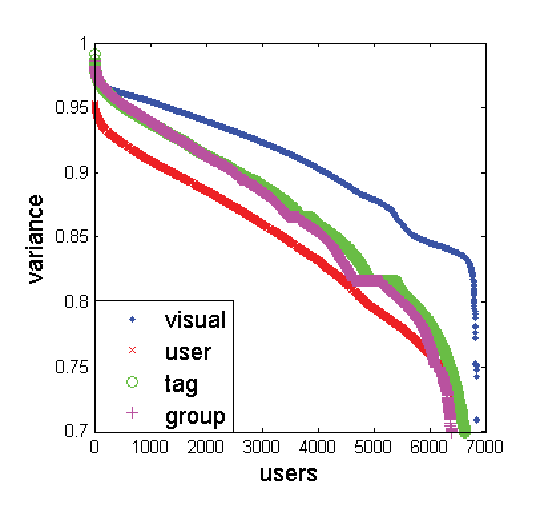
\epsfig{file=preliminary_1.eps, width=1.5in}
}
\subfigure[]{
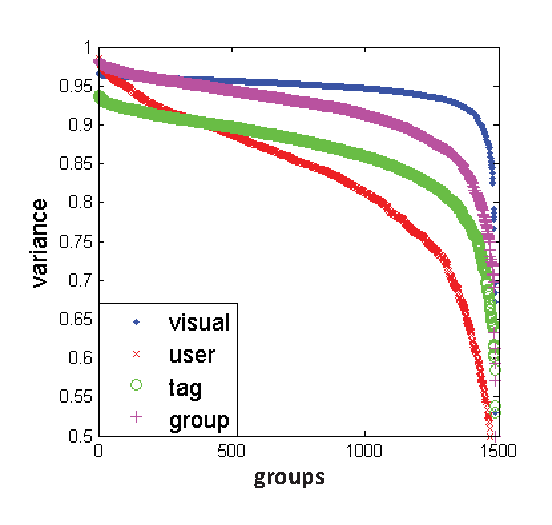
\epsfig{file=preliminary_2.eps, width=1.5in}}
\caption{The variance of the visual features and social factors of the images that are favored by each (a) user (b) group. The results are sorted in a descending order.}
\label{preliminary}\vspace{-0.3cm}
\end{figure}
\vspace{-0.2cm}\subsection{Reliability of Social Entities}
In social media, the user behavior information is usually noisy and uncertain. Thus not all social entities are equally reliable in evaluating social similarity. For example, images in the group named ``iphone club" should be similar but images in the groups named ``beautiful world" may be very diverse. In this case, the former group is more reliable than the latter one in similarity evaluation. Therefore, it is important to evaluate the reliability of social entities.

Take users as an example, if an image is favored by two users, we can assume that the interests of these two users are partially similar. Based on this assumption, we can build a similarity graph based on user interests. The nodes are users and the weight of an edge denotes the similarity of the users. We use $Im(v_i)$ to denote the images that are favored by user $v_i$, i.e.,
 \vspace{-0.1cm} \begin{equation} \vspace{-0.1cm}
 Im(v_i) = \{\mathcal{I}_t|v_i \in \mathcal{V}_t\}.
 \end{equation}
 In this equation, $\mathcal{V}_t$ denotes the all entities that belongs to image $\mathcal{I}_t$. Then, the similarity of the social entities can be defined as the Jaccard distance of the images:
 \vspace{-0.1cm} \begin{equation} \vspace{-0.1cm}
 sim(v_i, v_j) = \frac{|Im(v_i) \cap Im(v_j)|}{|Im(v_i)\cup Im(v_j)|}.
 \label{sim1}
 \end{equation}
 Based on the  similarity graph, we utilize spectral clustering method to divide users into $c$ clusters. For a given entity $v_i$, if all of its neighbors belong to the same cluster with $v_i$, we can think $v_i$ is a reliable social entity. The images belongs to user $v_i$ should have high probability to be similar. Thus, the reliability score of $v_i$  is defined as follows,
\vspace{-0.1cm} \begin{equation} \vspace{-0.1cm}
r(v_i) = \frac{1}{|c(v_i)\cup_{v_j \in N(v_i)} c(v_j)|},
\label{sp}
\end{equation}
where $N(v_i)$ is the set of neighbor nodes of $v_i$; $c(v_i)$ is the label of $v_i$'s cluster. If all of $v_i$'s neighbors  belong to the same cluster with it, the reliability score $r(v_i)$ is defined as $1$. On the contrary, if his neighbors cover all of $c$ clusters, $r(v_i)$ is defined as $1/c$.

This method is also suitable for the cases of using group or tag as social entity. For any entity $v_i$, the pair-wise similarity can be similarly calculated by Equation \ref{sim1} and the reliability score can be calculated by Equation \ref{sp}.
\vspace{-0.1cm}\subsection{Evaluation of Social Similarity}
We explore evaluating the social similarity of pair-wise images based on the reliability scores of the corresponding social entities. For two images $\mathcal{I}_i$ and $\mathcal{I}_j$, we analyze their similarity by their social factors $\mathcal{V}_i$ and $\mathcal{V}_j$. If $\mathcal{V}_i\cap \mathcal{V}_j$ is empty, i.e.,they share no common entities, we define the social similarity as 0. Otherwise, the social similarity is determined by the overlap of the entities and their reliability. Taking users as an example, intuitively, when the users have the same reliability, the images that are jointly favored by more users should be more similar. If the images are both favored by a fixed number of users, the images that are favored by more reliable users should have higher similarity. Based on the above two considerations, the social similarity of image in the social factor $\mathcal{V}_i$ and $\mathcal{V}_j$ is defined as follows,
\vspace{-0.1cm} \begin{equation} \vspace{-0.1cm}
sim(\mathcal{V}_i, \mathcal{V}_j) \!=\! \left\{\!\! \begin{array}{ll}
0, \!\!\!& \mathcal{V}_i \cap \mathcal{V}_j = \phi\\
\frac{\sum_{v_t\in \mathcal{V}_i \cap \mathcal{V}_j} r(v_t)}{\sum_{v_t \in \mathcal{V}_i \cup \mathcal{V}_j} r(v_t)}, \!\!\!& \textrm{otherwise}
\end{array}\right.
\label{sim2}
\end{equation}
where $r(v_t)$ is the reliability score defined in Equation \ref{sp}. In Equation \ref{sim2}, the similarity is defined as the weighted Jaccard similarity of $\mathcal{V}_i$ and $\mathcal{V}_j$. Obviously, this definition of similarity satisfies the previous heuristics. For a social image has multiple social factors, the final similarity of images $\mathcal{I}_i$ and $\mathcal{I}_j$ is defined as the average of all the social factors' similarity:
\vspace{-0.1cm} \begin{equation} \vspace{-0.1cm}
sim_{social}(\mathcal{I}_i, \mathcal{I}_j) = \frac{1}{m} \sum_{k=1}^m sim(\mathcal{V}^k_i, \mathcal{V}^k_j).
\label{social_sim}
\end{equation}
In this equation, we use average because different social factors reflect different aspects of image similarity. The final social similarity values range from 0 to 1. When the similarity is close to 1, the images are judged very similar in social dimension. On the other hand, when the similarity is near to 0, we are not very certain that the images are very dissimilar because similar images may also have no social relation. This problem can be solved by multiple sampling. Because of the diversity of the images, for a given image, if we randomly select many socially dissimilar images, the vast majority of them will be truly dissimilar to it.

\vspace{-0.2cm}\section{SOCIAL EMBEDDING IMAGE DISTANCE LEARNING} \label{sec_app}

When social similarity of images is estimated, our target is to learn an image distance function to reduce the distance of socially similar image and enlarge the distance of socially dissimilar images. In this section, we first introduce our proposed image distance learning method. Next, we give the algorithm of our approach and analyze the complexity. Finally, we design two applications based on the proposed image distance metric, including image recommendation and text-based image reranking.

\vspace{-0.1cm}\subsection{Mahanalobis Distance Function}
%ͨ��ŷ�Ͼ����������Ͼ��� ���ܻ���֪ʶ
In traditional metric learning researches, \emph{Mahalanobis} Distance is a widely used metric function because it is very efficient in optimization and calculation, as well as effective enough in most problems. Although some kernel functions are proposed to improve the performance. We do not consider them because the metric function is not the main contribution of this work and it may make our method not scalable. Therefore, we use \emph{Mahalanobis} Distance to evaluate the image distance, which is defined as follows,
\vspace{-0.1cm} \begin{equation} \vspace{-0.1cm}
d_M(\mathnormal{x}_i, \mathnormal{x}_j) = \sqrt{(\mathnormal{x}_i - \mathnormal{x}_j)^TM(\mathnormal{x}_i - \mathnormal{x}_j)},
\label{distance}
\end{equation}
where $M$ is the \emph{Mahalanobis} matrix, which needs to be learned in our problem; $\mathnormal{x}_i$ is the  visual feature vector of image $\mathcal{I}_i$. To guarantee $d$ to be a distance function, $M$ must be positive semidefinite, which is noted as $M \succeq 0$.

%For $M\in R^{n \times n}$, there exists $L\in R^{n \times n}$, which makes $M=L^TL$. Thus, Equation \ref{distance} can be written as:
%\vspace{-0.1cm} \begin{equation} \vspace{-0.1cm}
%d_M(\mathnormal{x}_i, \mathnormal{x}_j) = \sqrt{(\mathnormal{y}_i - \mathnormal{y}_j)^T(\mathnormal{y}_i - \mathnormal{y}_j)},
%\label{distance2}
%\end{equation}
%where $\mathnormal{y}_i = L\cdot \mathnormal{x}_i$. From Equation \ref{distance2}, we can easily observe that \emph{Mahalanobis} distance actually linearly maps original visual space to a new space.

\vspace{-0.1cm}\subsection{Distance Learning with Social Constraints}
In our metric learning approach, our goal is to learn the \emph{Mahanalobis} matrix $M$ from the social images, which makes the image distance $d_M(\mathnormal{x}_i, \mathnormal{x}_j)$ consistent to social similarity. i.e., the distance between socially similar images is close and the distance between socially dissimilar images is far.

In metric learning, ``triple" is a widely used concept for optimization. In our approach, a ``triple" $<i, j, k>$ is defined as three images $I_i, I_j$ and $I_k$, where $I_i$ and $I_j$ are socially similar and $I_i$ and $I_k$ are socially dissimilar. Thus, we can train our metric function by reducing $d_M(\mathnormal{x}_i, \mathnormal{x}_j)$ and enlarging $d_M(\mathnormal{x}_i, \mathnormal{x}_k)$. In our method, the training set of triples $\mathcal{T}$ based on social similarities is defined as:
\begin{equation}
\mathcal{T} = \{<i, j, k>|sim_{social}(\mathcal{I}_i, \mathcal{I}_j) >\delta, sim_{social}(\mathcal{I}_i, \mathcal{I}_k) < \epsilon \},
\label{triple}
\end{equation}
where $\delta$ and $\epsilon$ are the thresholds to specify socially similar images and socially dissimilar images. In social media, there are a lot of socially dissimilar images and a few socially similar images. For a given $<x_i, x_j>$, there are a lot of $x_k$ that satisfies the equation \ref{triple}. In our approach we just randomly select some of them to avoid explosion of scale and reduce the redundancy. After the set of of triples $\mathcal{T}$ is selected, we need to find the optimal \emph{Mahanalobis} matrix $M$ that satisfies the following constraints:
\begin{equation}
d^2_M (x_i, x_k) - d^2_M (x_i, x_j) > 1, \forall <i,j,k> \in \mathcal{T}
\label{cons1}
\end{equation}\vspace{-0.1cm}
Following the traditional margin-based metric learning methods\cite{lmnn, nips03}, the margin between two distances is defined as the squared error because it is very easy to optimize and have a good performance. In Equation \ref{cons1}, the matrix $M$ that satisfies all the constraints is typically not unique. In this case, we aim to select $M$ that is close to the original unweighted Euclidean Distance, which represents the original visual similarity in our problem. This leads to the following optimization problem:
\vspace{-0.1cm} \begin{equation} \vspace{-0.1cm}\label{problem1}
\begin{split}
&\min_M ||M-I||^2_F\\
s.t. \quad & d^2_M (x_i, x_k) - d^2_M (x_i, x_j) > 1, \forall <i,j,k> \in \mathcal{T}\\
&M \succeq 0
\end{split}
\end{equation}\vspace{-0.1cm}

where $I$ is the identity matrix with the same dimensions with $M$ and $||\cdot||_F$ donotes \emph{Frobenius} norm. As in other margin-based methods, we add slack variables \cite{slack} to account for the constraints that cannot be satisfied. Thus our problem can be written as follows,
\vspace{-0.1cm} \begin{equation} \vspace{-0.1cm}\label{problem2}
\begin{split}
&\min_M ||M-I||^2_F + C \sum_{i,j,k}sim_{social}(\mathcal{I}_i, \mathcal{I}_j)\epsilon_{ijk}\\
s.t. \quad & d^2_M (x_i, x_k) - d^2_M (x_i, x_j) > 1 - \epsilon_{ijk}, \forall <i,j,k> \in \mathcal{T}\\
&M \succeq 0, \quad \epsilon_{ijk} \geq 0
\end{split}
\end{equation}\vspace{-0.1cm}
where $\epsilon_{ijk}$ is the slack variable and $sim_{social}(\mathcal{I}_i, \mathcal{I}_j)$ is the social similarity defined in Equation \ref{social_sim}. $C$ is a parameter that denotes the  stringency of the slack variables. Different from traditional methods, we use social similarity as the coefficient of the slack variables because we have different confidence for different training triples. When the images $\mathcal{I}_i$ and $\mathcal{I}_j$ are very socially similar, i.e. $sim_social(\mathcal{I}_i, \mathcal{I}_j)$ is close to 1, we hope the corresponding constraint to be satisfied as far as possible. On the contrary, when $sim_{social}(\mathcal{I}_i, \mathcal{I}_j)$ is very small, the value of slack variable can be relatively greater. This problem is a Semi-Definite Programming (SDP) problem. It can be solved by the existing solvers \cite{sedumi}.

\vspace{-0.1cm}\subsection{Algorithm and Complexity}
We summarize the procedure of the whole Social Embedding Image Distance Learning approach as described in Algorithm \ref{alg1}.

\begin{algorithm}[htb] %�㷨��ʼ
\caption{Social embedding Image Distance Learning}
\label{alg1}
\small
\KwIn
{the number of the social factors $m$;\\
the number of social entities in the $i^{th}$ social factor $f_i$;\\
the number of the training images $n$;\\
the visual features $x_i$ and social factors $\mathcal{S}_i=\cup_{k=1}^m \mathcal{V}_i^k$ for each training image $\mathcal{I}_i$}
\KwOut{
the \emph{Mahanalobis} matrix $M$ for the distance metric in Equation \ref{distance}.}
\For{ ($i=1:m$) }{ %���濪ʼ���㷨������
    \For {$j=1:f_i -1$}{
        \For {$k=k+1:f_i$}{
            {Compute the pair-wise similarity of social entity $sim(v_i^j, v_i^k)$ using Equation \ref{sim1}\; }}}
     {Conduct spectral clustering on the similarity graph\;}
    { Compute the reliability score of the social entity $v_i^k$ using Equation \ref{sp}\;}}
\For{($i=1:n-1$)}{
    \For {$j = i+1 :n$}{
        { Compute the social similarity of the training images $sim(I_i, I_j)$ using Equation \ref{social_sim}\;}}}
{{$\mathcal{T} = \Phi$\;}}
\For{ $i=1:n$}{
    \For { $j \in \{j|sim(I_i, I_j) > \delta\}$}{
        \For {t=1:r}{
             {Randomly generate $k \in \{1, 2, \cdots, n\}$, $sim(I_i, I_k) < \epsilon$\;}
             {Add $<i,j,k>$ to $\mathcal{T}$\;}}}}
{Formulate the Problem in Equation \ref{problem2}\;}
{Optimize the SDP problem by standard solvers\;}
\end{algorithm}

There are four main steps in our approach: entity reliability evaluation step, social similarity computation step, triple selection step, and optimization step. In entity reliability evaluation step, the time complexity is $\mathcal{O}(\sum_{i=1}^m f_i^2)$,  $m$ is the number of social factors and $f_i$ is the size of the $i^{th}$ social factor. In social similarity computation step, the complexity is $\mathcal{O}(n^2m)$. In the triple selection step, the time complexity is $\mathcal{O}(r\cdot \sum_{i=1}^n |S_i|)$, where $n$ is the total number of the training images,  $|S_i|$ is the number of the images that are socially similar to the $i^{th}$ image and $r$ is a constant that denotes the number of socially dissimilar images sampled. Usually, we have $|S_i| << n$, thus the complexity of this step is usually much less than $\mathcal{O}(n^2 r)$. In the last optimization step, the complexity of SDP is $\mathcal{O}(c|T|)$, where $c$ is a constant that is determined by the number of iteration and the length of visual features, as well as $|T|$ denotes the number of selected triples. At the same time, we have $|T| \leq n^2 r$. Based on the above analysis, the total complexity  of our algorithm is no more than $\mathcal{O}(crn^2)$. Therefore, the time complexity of our algorithm is square with respect to the number of training images.

\vspace{-0.2cm}\subsection{Applications}
In image search and recommendation tasks, human cognition plays an important role. Thus, our approach is very useful in these tasks. In this section, we introduce how and why our image distance metric can be used in the corresponding application scenarios.
\vspace{-0.1cm}\subsubsection{Image recommendation}
In the image recommendation task, our target is to recommend new images based on his/her historical browsing logs. In our approach, we learn the image distance function from users in social platforms. Then, for general Web images, we can judge whether two images will have similar favored users according to their visual contents. Given a set of images $Train = \{I_1, I_2, \cdots, I_m\}$ that have been viewed by the current user, we need to recommend the top $k$ images in the candidate set $Test = \{J_1, J_2, \cdots, J_n\}$. Intuitively, the image that are similar to the images in $Train$ should be recommended. In our distance learning method, when the optimal \emph{Mahanalobis} matrix $M$ is obtained, the pair-wise image distance $d_M(I_i, I_j)$ can be calculated accordingly. Thus, the next question is how to select the images that are similar to the training set based on the distance function. Here we provide the Borda Fusion model to solve the problem.

Borda Count has been widely used in meta-search and recommendation \cite{borda}. It simulates a democratic voting process: each voter gives a preference rank to $d$ candidates; the top ranked candidate gets $d$ points, the second ranked one gets $d-1$ points and so on so forth. Then, for each candidate, the total points from all voters are used for ranking. The top $k$ results are returned for recommendation. In this model, each image in the training data is regarded as a voter. For each training image, we calculate the distance from it to the testing images $J_q$ in $Test$. Then, the distance $d_M(I_p, J_q)$ are ranked in ascending order. The top $d$ test images obtain their points. Finally, after all the training images in $Train$ are traversed, we rank the testing images in $Test$ with respect to their total points. We return the top $k$ images as the recommendation results.

To notice, our recommendation process is purely content-based. Thus, in this paper, we do not compare our method to other user-centric recommendation methods such as \emph{Collaborative Filtering (CF)} because we do not need any user information.  In addition, as CF suffers from cold-start problem, hybrid recommendation (e.g. CF+content-based) becomes more popular, where image distance metric is also a fundamental problem.
\vspace{-0.3cm}\subsubsection{Image reranking}
When people search a query in the image search website, the search engine will return a lot of images that are judged as relevant to the query.  Reranking the images to better meet the demands of users is an important problem. Jing \emph{et al.} \cite{visualrank} proposed a VisualRank method for image reranking. In this method, the similarity of two images are evaluated by their visual features. Then, a PageRank \cite{pagerank} based iterative calculation is conducted to give the images rank scores. This method selects the images that are visually similar to most of the other images. It has been proven that VisualRank performs well in product search. However, in general image search task, the performance is not very desirable because it ignores human cognition factor. Our approach learns the social similarity, which can better estimate human cognition. In our approach, the pair-wise image similarity is evaluated by the learned distance function $d_M(\mathcal{I}_i, \mathcal{I}_j)$. The PageRank model is used to select the images that are interesting to most of the users.

 In this method, we first generate the image similarity matrix $P$, whose elements are calculated as:
\vspace{-0.1cm} \begin{equation} \vspace{-0.1cm}
P_{ij} = \frac{e^{-d_M(\mathnormal{x}_i, \mathnormal{x}_j)}}{\sum_{k=1}^n e^{-d_M(\mathnormal{x}_k, \mathnormal{x}_j)}}
\end{equation}
where $d_M(\mathnormal{x}_i, \mathnormal{x}_j)$ is the learned \emph{Mahanalobis} distance in Equation \ref{distance}, $n$ is the number of candidate images. Here we use negative exponent function to convert distance to similarity and chose $\sigma^2 = 0.5$. The denominator aims at normalizing the sum of each column to 1. Then, the PageRank process is conducted:
\vspace{-0.1cm} \begin{equation} \vspace{-0.1cm}\label{reranking_eq}
\mathnormal{pr} = d\cdot P\cdot \mathnormal{pr} + (1-d)\mathnormal{e}
\end{equation}
where $\mathnormal{pr}$ denotes the rank score vector, $d$ is the damping factor to guarantee the connectivity of the similarity graph, and $e$ is a normalized $n$-dimension vector whose elements are all $1/n$. In PageRank, the empirical value of $d$ is about $0.8$. After the PageRank process, each image has a rank score in $\mathnormal{pr}$. Finally we can rerank images by their rank scores.



\vspace{-0.3cm}\section{EXPERIMENTS} \label{experiments}
In this section, we first introduce our experimental settings. Then we evaluate the proposed approach in three aspects: the effectiveness of our learning method, as well as the performance of the learned distance function in recommendation task and image reranking task. Finally, we show some learning results and give some interesting insights of our distance learning method.
\vspace{-0.2cm}\subsection{Experimental Setup}
\subsubsection{Datasets}
In our experiments, we have prepared three datasets, including:

\textbf{Training dataset and test dataset.} To train the distance function and test the effectiveness of our distance learning method, we crawl the images and their social contextual information in Flickr through Flickr API. This dataset includes 101,496 images, 54,173 users, 6,439 groups and 35,844 tags in total. We crawl the data by the following criteria: first, we search for 500 hot queries\footnote{https://www.flickr.com/photos/tags/.}, such as sunset, portrait, etc. to obtain the seed images. Then the images that belong to the same user or group with the seed images are expanded. We crawl the social information of the images, including: the users who favor them, the groups that the images belong to, as well as the tags annotated to the images. Some images may have no favored users or interest groups. We divide this dataset into two parts: 80\% for training and 20\% for test.The social entities in the training and test datasets may have overlap. It will not impact the fairness of our experiments because we do not evaluate the similarity between training and test data in our method.

\textbf{Recommendation dataset.} We also prepare a recommendation dataset for the application scenario of image recommendation. We select 1,793 users' favorite images in Flickr. The users selected must have at least 40 favorite images. For each user, we randomly select 20 images for training and 20 as ground truth for testing. Then we sample other 80 images from the whole image dataset as candidates. Each candidate image must have at least one tag that is the same as one of the ground truth images.

\textbf{MSR dataset.} We utilize Bing Image Retrieval Grand Challenge (MSR) dataset \cite{click_bing} to prove that our distance learning method can improve the performance of image reranking.  Different from traditional image retrieval datesets, MSR dataset is based on user click data, which can capture not only semantic relevance but also human cognition.

The first two datasets are crawled from Flickr because our methods rely on social behavioral infomation. However, to the best of our knowledge, there is no public benchmark including such information. In our image reranking method, we do not need any personalized information. Thus a public dataset is utilized to make our approach comparable to others.

\vspace{-0.2cm}\subsubsection{Visual Features}
Visual feature is an important setting in our method because it determines the performance of transfer learning. If there is no relationship between the used visual feature and the social similarity of the images, our method will not work. Although using multiple features may improve the performance, it will bring much higher complexity at the same time. The key point of this paper is distance learning but not feature selection. Therefore, we only use a simple and effective visual feature in our experiments. In our approach, local features are better than global features because local features represent images in object level, which can better reflect user interests.  Among the various local features, we utilize a Bag-of-Words (BoW) histogram based on SIFT descriptors \cite{bow, sift} in our experiments, which is one of the most widely used presentation of images. The SIFT descriptors are extracted by a VLFeat implementation \cite{vlfeat}. Then a hierarchical $k$-means visual vocabulary tree is constructed with 4 layers and 10 branches for each layer. After clustering, each leaf node in the vocabulary tree is defined as a visual word. An image is presented as the histogram of the visual words occurred. In our datasets, all images are rescaled to the normal size in Flickr for uniformity: the length of the longest edge is rescaled to 400 pixels.

\vspace{-0.2cm}\subsubsection{Baselines}
To demonstrate the advantages of our proposed distance learning approach \emph{SIDL}, we implement the following baseline methods for comparison.

(1) \textbf{Euclidean distance.} When the BoW features are extracted, the Euclidean distance is commonly used to evaluate the image distance, i.e.:
\vspace{-0.1cm} \begin{equation} \vspace{-0.1cm}
d(x_i, x_j) = \sqrt{(x_i-x_j)^T (x_i - x_j)}.
\end{equation}

(2) \textbf{Jaccard similarity.} If we regard an image as a document, when it is presented as a bag of words, the Jaccard distance \cite{jaccard}, which is a set similarity function for documents can also be utilized:
\vspace{-0.1cm} \begin{equation} \vspace{-0.1cm}
sim(I_i,I_j) = \frac{|I_i \cap I_j|}{|I_i \cup I_j|},
\end{equation}
where $I_i$ denotes the $i^{th}$ image that is presented as a set of visual words. For it is a similarity function, we convert it to distance by negative exponent function if needed.

(3) \textbf{TagProp \cite{tagprop}.} Guillaumin \emph{et al.} proposed a method named \emph{TagProp}  for image annotation. This method use metric learning technology to learn the image distance with respect to their tags.  Although the final output of this method is the tag relevance, it evaluates the pair-wise image similarity in the optimization process. In our experiments, we only use the results of image distance.

(4) \textbf{LMNN \cite{lmnn}.} Weinberger \emph{et al.} proposed a metric learning method named Large Margin Nearest Neighbor (LMNN). \emph{LMNN} uses metric learning to reduce the margins of the nearest neighbors. It is designed for image classification, which relies on the pre-labeled data. For our training data do not contain the label of classification, we use the image classification benchmark Caltech101 \cite{c101} as the training dataset, which includes 102 categories, and 40 to 800 images per category. We select 30 images per category for training. Then, the trained \emph{Mahanalobis} distance function is compared to our method.

(5) \textbf{social+LMNN.} In this baseline, we use the social similarity estimation in Equation \ref{social_sim} to select the nearest neighbor of an image, and then use \emph{LMNN} for optimization. Here we use this as a baseline to compare the metric learning optimization step in the same condition of social similarity estimation.

In the area of image processing, there are a variety of methods for image search and recommendation. However, in this paper, we only want to prove that our cognition-based image distance performs better than the traditional image distance metrics. Thus we fix the Borda Fusion model in recommendation and PageRank model in reranking and use the above distance metrics as baselines.


The code of our algorithm is realized in MATLAB 2010b. The toolbox of VLFeat \cite{vlfeat} is used for SIFT feature extraction and hierarchical $k$-means clustering of visual words. We use SeDuMi \cite{sedumi} toolbox as the solver of the proposed optimization problem.  All the experiments were conducted on a server with Intel(R) Xeon(R) CPU X5645 at 2.40 GHz on 24 cores, 192GB RAM and 64-bit Windows Server 2008 operating system.

%��Ҫע�� ����������recommendation����search�ķ����ȣ���Ϊ������Ҫ֤������distance learning����Ч�ԡ�
\vspace{-0.2cm}\subsection{Effectiveness of SIDL}
The goal of our approach is to learn the social similarity in visual space. Thus, we first need to prove the feasibility of this idea. When we have learned a distance function from the training set, can this function reflect the social similarity in the test data? Here we evaluate the effectiveness in ranking because ranking order is much more important than absolute value in our problem. For a given image in the test dataset, we calculate the social similarity to the other images by Equation \ref{social_sim} and then can obtain a rank order as ground truth. On the other hand, we can calculate the image distance based on the learned distance function by Equation \ref{distance} and get another rank order of similar images. The consistency of these two orders can reflect the effectiveness of our method. We use $Kendall-\tau$ rank correlation \cite{tau} as the evaluation measure. Give two ranking sequence $X$ and $Y$. The $Kendall-\tau$ is defined as:
\vspace{-0.1cm} \begin{equation} \vspace{-0.1cm}
\tau = \frac{n_c - n_d}{\frac{1}{2}n(n-1)},
\end{equation}
where $n$ is the total number of images, $n_c$ is the number of concordant pairs and $n_d$ is the number of discordant pairs. A concordant is defined as the pair $(i, j)$ that satisfies $x_i \geq x_j$ when $y_i \geq y_j$ or $x_i \leq x_j$ when $y_i \leq y_j$. Otherwise, $(i,j)$ is a discordant pair. The scale of $Kendall-\tau$'s value is $[-1,1]$. If $X$ and $Y$ are the same, $\tau = 1$. If $X$ and $Y$ are completely inverted, $\tau=-1$.

%�������۷���������ָ��
In training process, we fix the value of $\delta$ and $\epsilon$ in Equation \ref{triple} as $\delta=0.7, \epsilon=0.1$. In this setting, an image in the training dataset has 179 socially similar images and about 70,000 socially dissimilar images in average. To reduce the complexity of our optimization process, for each image, we randomly select 200 socially dissimilar images in the triple selection step in Equation \ref{triple}. We use a 5-folds cross validation to tune the parameter $C$ in the Equation \ref{problem2}. The best performance of $\tau$ is obtained when $C=0.15$.

In social similarity evaluation step, we need to discover what social factors are helpful in evaluating  social similarity. Therefore, before comparing our methods to the baselines, we first use different social factors to demonstrate their effects on the final performance. Figure \ref{effective_factor} illustrates the results.
%��������C=0.15 ��ͼ���Ͳ���social factor �Աȸ�ͼ
\begin{figure}
\centering
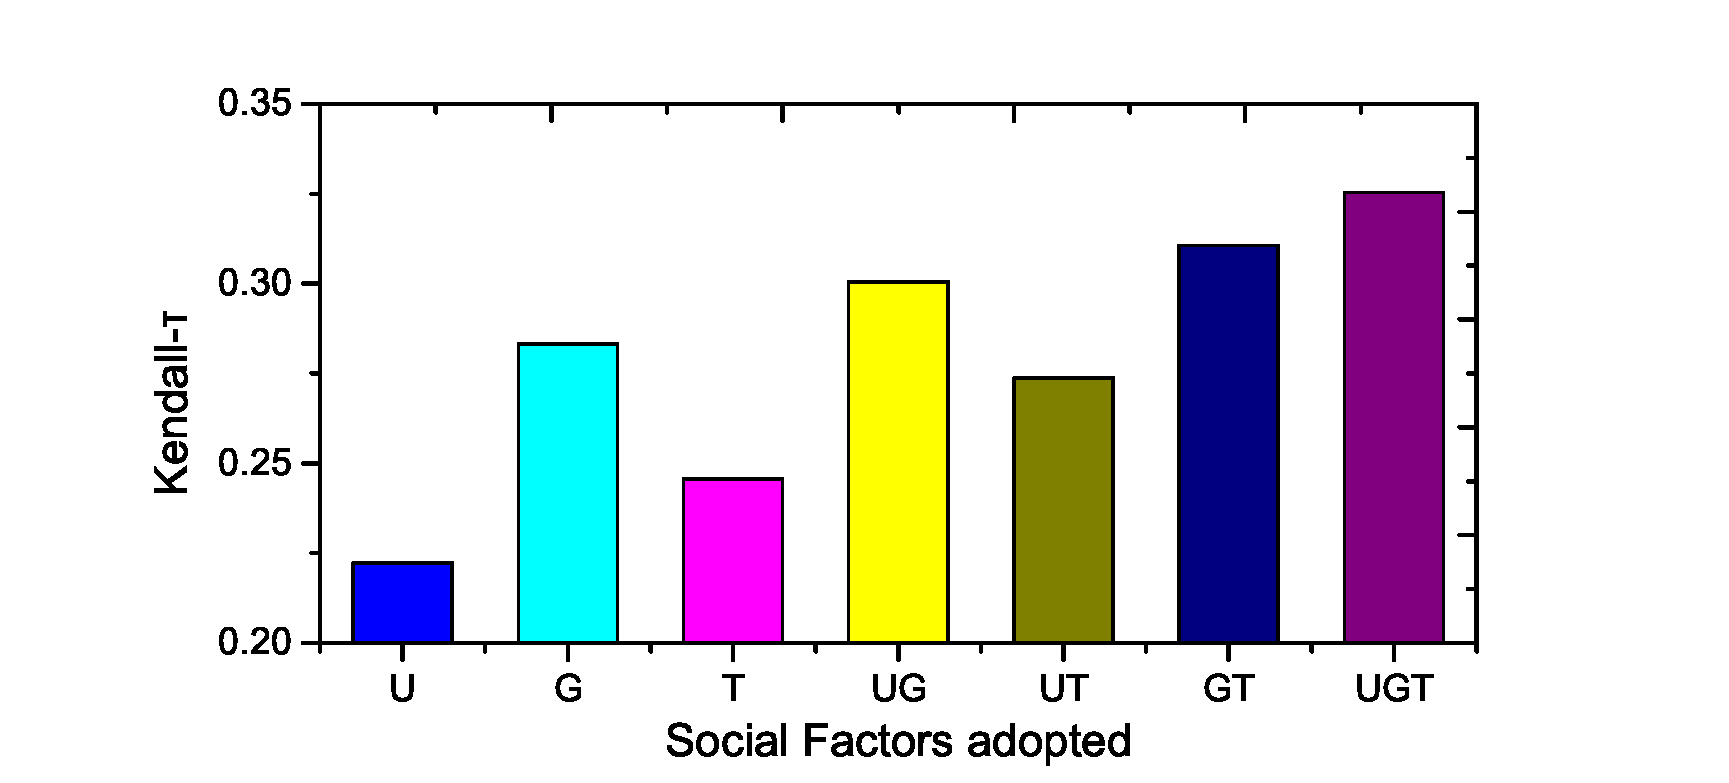
\epsfig{file=effective_factor.eps, width=3in}
\caption{The Performance on the test dataset in $Kendall-\tau$ using different social factors. ``U" denotes users, ``G" denotes groups and ``T" denotes tags.  }
\label{effective_factor}
\vspace{-0.3cm}\end{figure}

Figure \ref{effective_factor} is generated by using different social factors to calculate the social similarity in Equation \ref{social_sim}. In Figure \ref{effective_factor}, ``U" denotes users, ``G" denotes groups, ``T" denotes tags and multiple symbols denotes using multiple social factors. When we use different factors, the value of $\delta$ and $\epsilon$ are adjusted at the same time to guarantee that the number of socially similar images is about 200 and the number of socially dissimilar images is about 70,000. In Figure \ref{effective_factor}, we can observe that our algorithm obtains the best performance when using ``UGT". It shows that all these factors are helpful to improve the performance. If we only use one factor, group is the best and user is the worst. This is because images in the same group are relatively concentrated in user interests but the images belong to the same user sometimes may be very diverse.   If we use two social factors, the best performance is obtained when using groups and tags. It is interesting that using group and user also has a not bad performance. It reflects that the knowledge of group and user has less overlap than  group and tag.

We compare our method to the baselines to demonstrate the effectiveness. The results are illustrated in Figure \ref{effective_perform}.
\begin{figure}
\centering
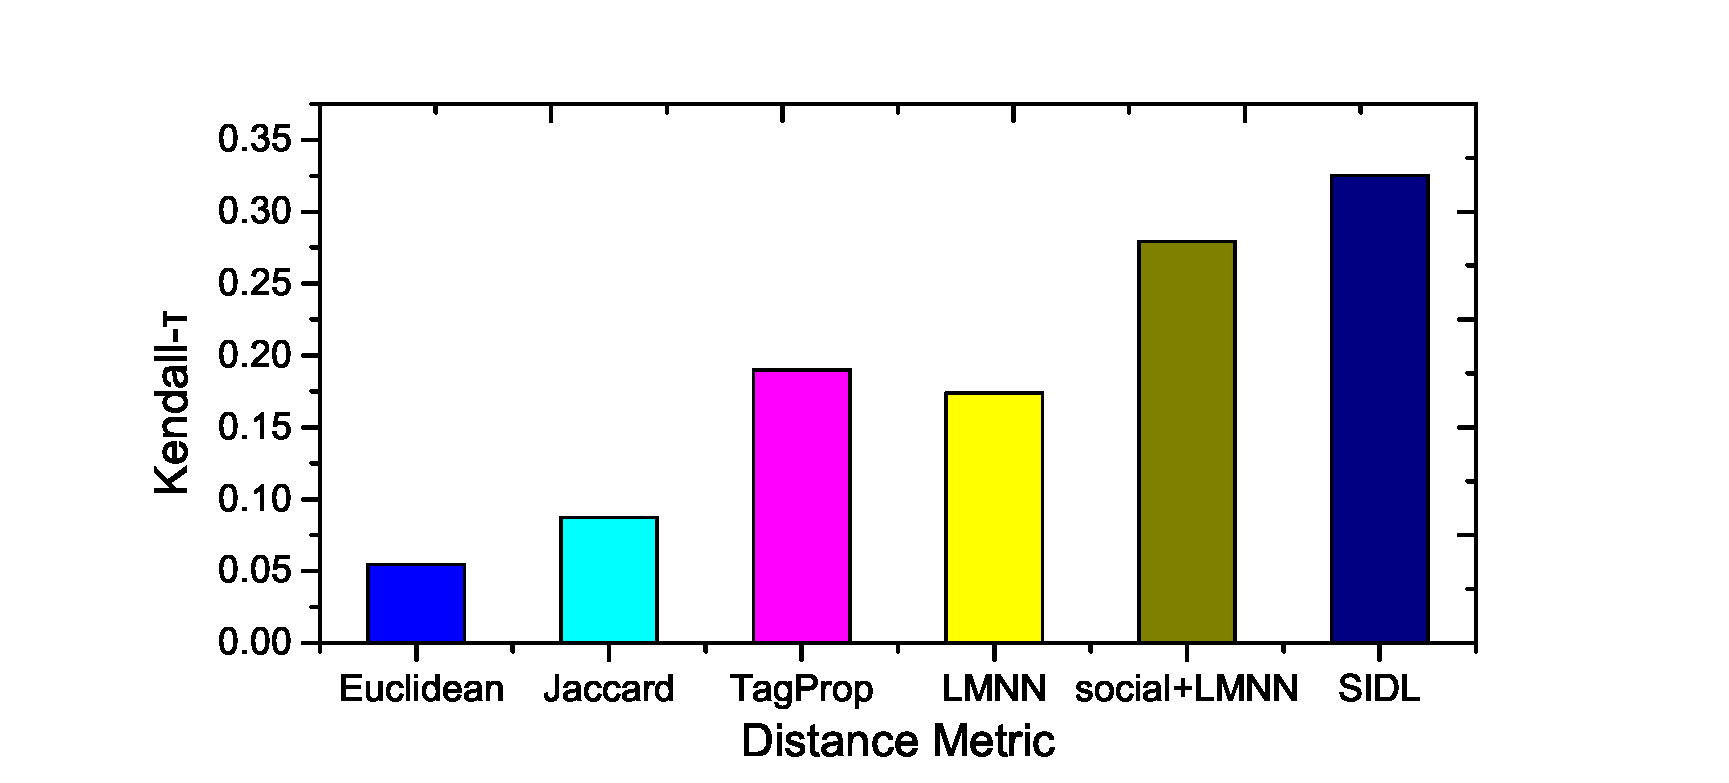
\epsfig{file=effective_perform.eps, width=3in}
\caption{The performance on the test dataset in $Kendall-\tau$ of different image distance metrics.  }
\label{effective_perform}
\vspace{-0.3cm}\end{figure}
%��baseline�Աȸ�ͼ
From Figure \ref{effective_perform}, it can be observed that the proposed \emph{SIDL} method achieves the best performance. In baseline methods, Euclidean distance and Jaccard similarity are unsupervised. The $\tau$ values of these metrics are less than 0.1, which means the rank orders are likely to be random.  \emph{LMNN} performs the worst among the four supervised methods. It is mainly due to the difference in the training datasets. In Flickr, most of the images are usually informal and noisy. However, images in Caltech101 dataset is well structured and have obvious objects. Besides, the amount of images in Caltech101 is only about $1/10$ scale of our Flickr training dataset.  The fact that \emph{social+LMNN} performs better than \emph{TagProp} shows that tag similarity in the training data cannot represent social similarity in the test data well.

Both \emph{social+LMNN} and \emph{SIDL} use social and visual information. The difference between these two methods exists in the optimization step. In the training dataset, an image usually only has less than 200 socially similar images. Compared to the total 80,000 images, socially similarity is very sparse. Thus if two visual words A and B do not occur in any pair of socially similar images, we can learn nothing in metric learning process.  In \emph{SIDL}, we initialize the distance function as the Euclidean distance, for the images whose distance cannot be learned, their visual similarity is maintained. Besides, in Equation \ref{problem2}, we add reliability scores as coefficients to the relax variables, which can make the constraints of highly similar pairs more accurate.

In this experiment, all the testing ground truth are based on the social similarity defined in Equation \ref{social_sim} because we only want to prove that it is effective to learn image distance of visual features from social similarity.  Thus we will demonstrate the effectiveness of our approach in real applications in the next section.
\vspace{-0.2cm}\subsection{Performance in Image Recommendation and Image Reranking}
Here we first show the performance of our method in the image recommendation task. In the image recommendation dataset, each user has $20$ images for training and $100$ for testing. In the $100$ testing images, $20$ should be recommended. For each image distance metric, we use the Borda Fusion model in Section \ref{sec_app} to calculate the voting points of the testing images according to their distance to the training images. Top $k$ images are returned as the recommendation results. Here we use $Precision@k$ and $Recall@k$ as the measures. The results are illustrated in Figure \ref{recommend}.
\begin{figure}
\centering
\subfigure[Precision]{
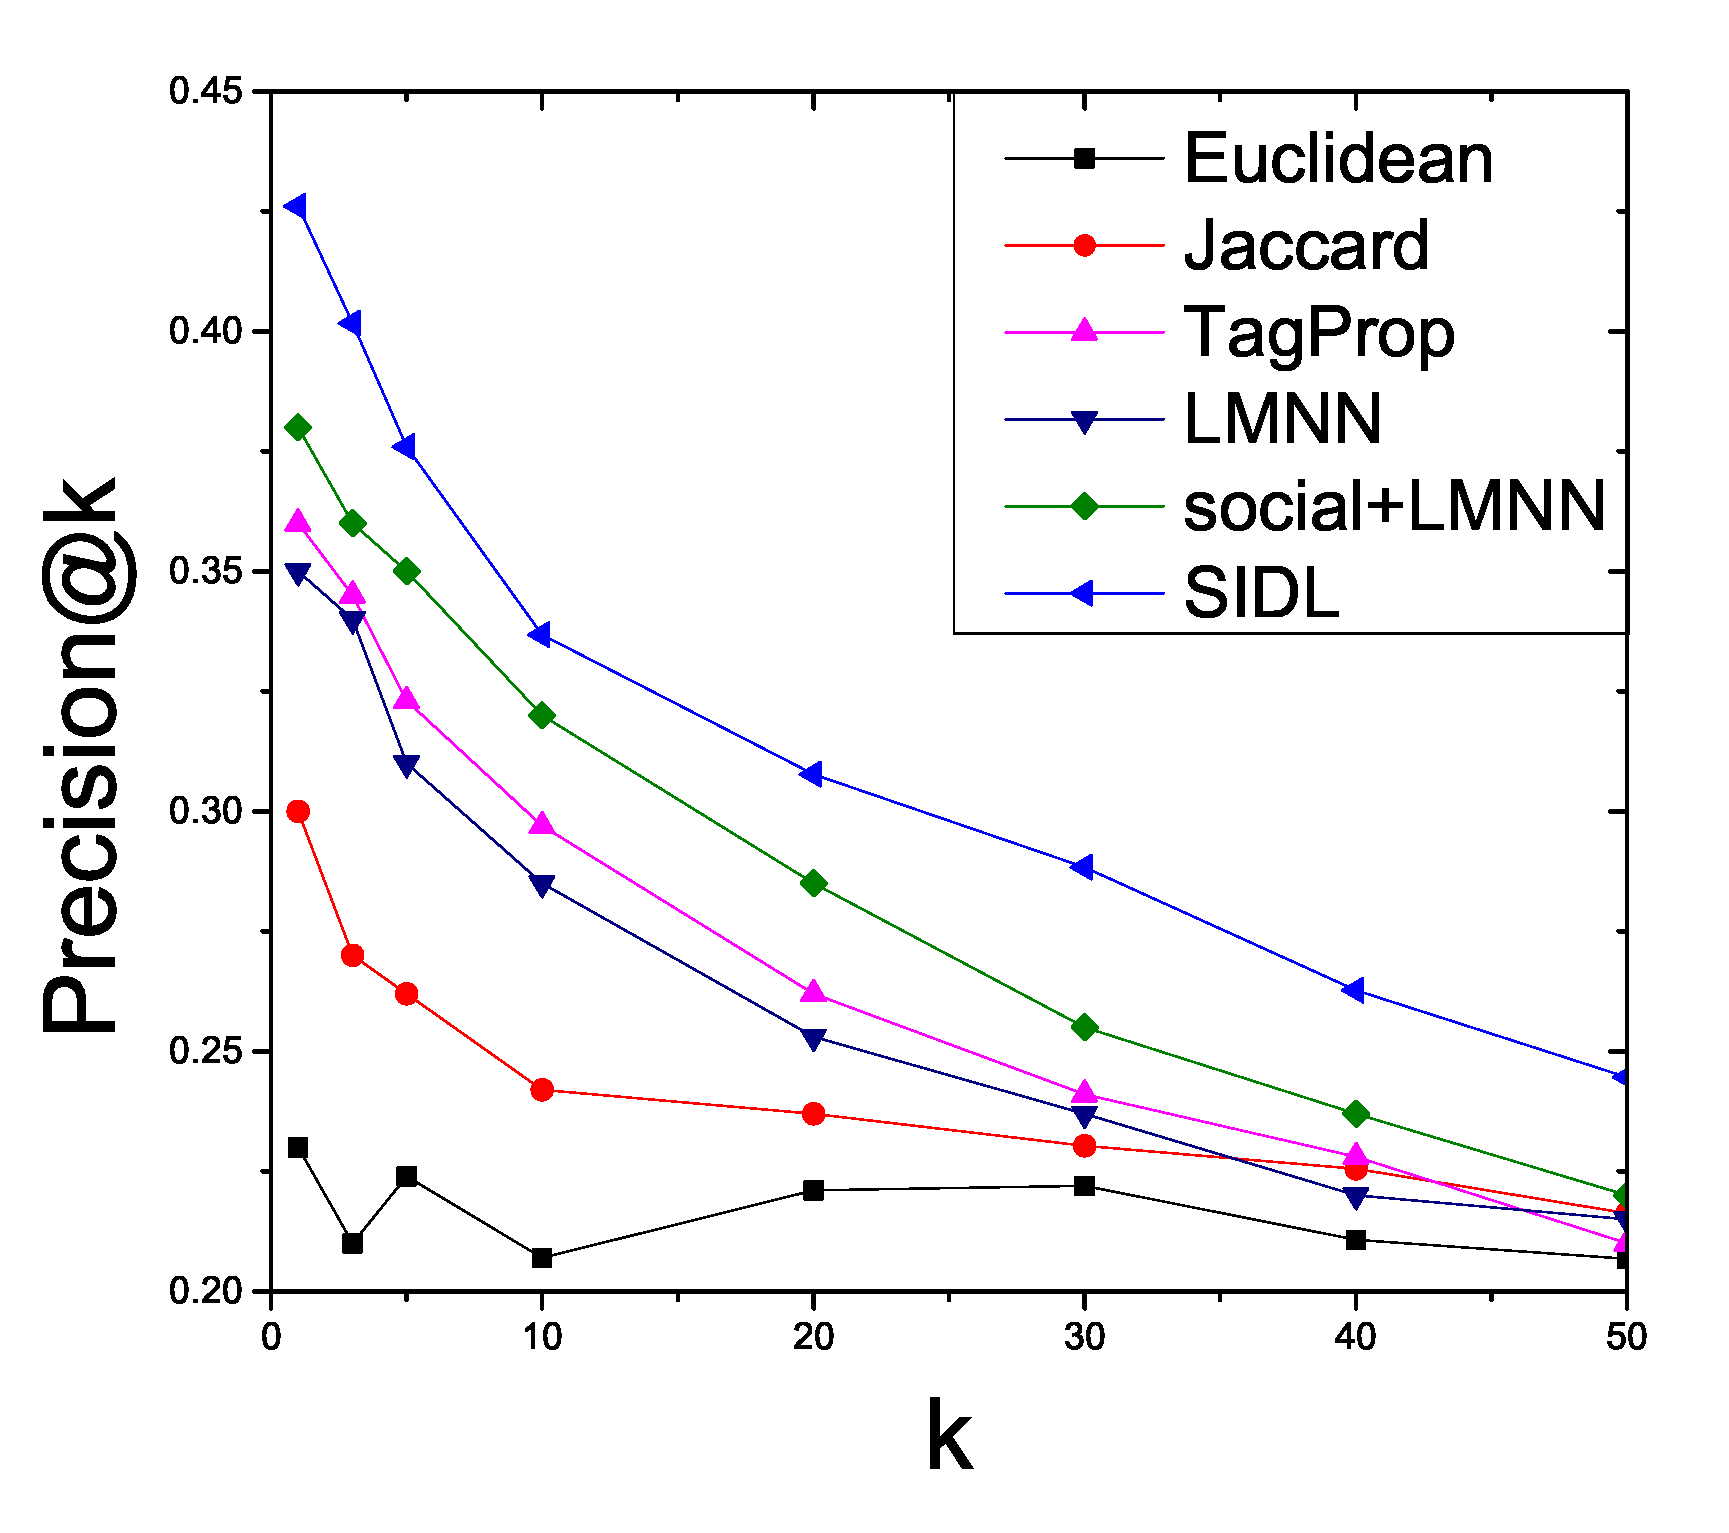
\epsfig{file=recommend_precision.eps, width=1.5in}
}
\subfigure[Recall]{
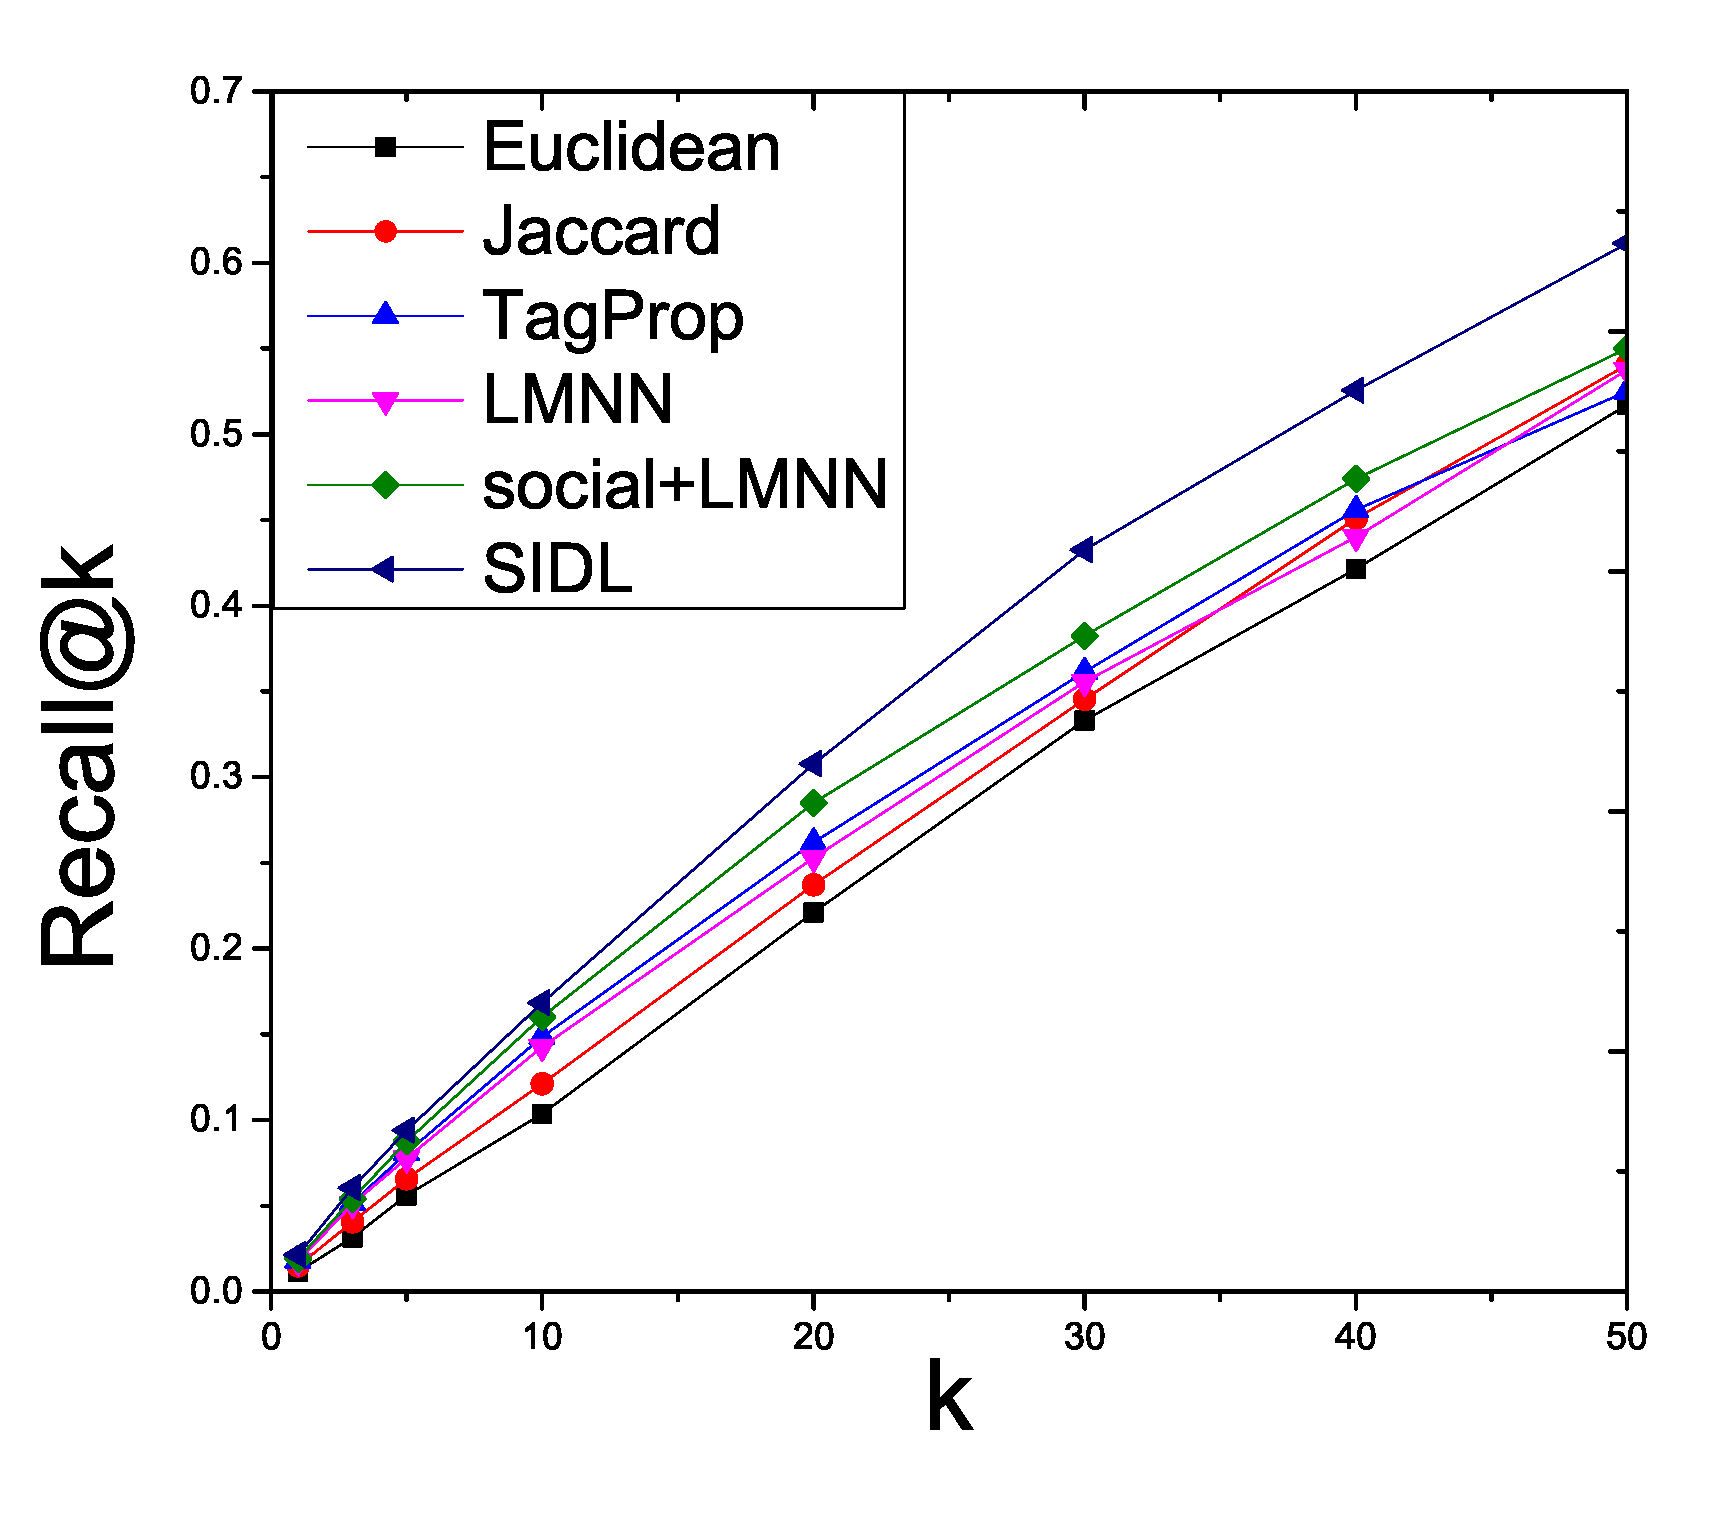
\epsfig{file=recommend_recall.eps, width=1.5in}
}
\caption{The performance on recommendation dataset in (a) Precision@k and (b) Recall@k with different number of top $k$ images using different image distance metrics in our Borda-fushion based image recommendation model. }
\label{recommend}
\vspace{-0.3cm}\end{figure}
In the figure, it can be seen that  \emph{SIDL} performs the best in both Precision and Recall for all $k$ values. If we recommend images randomly, the precision will be $0.2$. Similar to the last experiment, the result of Euclidean is near to random, which indicates the Euclidean distance of BoW features can hardly reflect the image similarity in recommendation task. The relative performance of the baselines is similar to the previous experiment except for \emph{LMNN} and \emph{TagProp}. In recommendation dataset, \emph{LMNN} performs better than \emph{TagProp}, which indicates the general category information might be effective than the specific tag information in recommendation task. Compared to \emph{social+LMNN}, \emph{SIDL} performs 10\% higher in Precision. It indicates the proposed metric learning optimization method has superiority to traditional \emph{LMNN} in embedding social information.

To show the performance in the image reranking task, we use different distance metrics in the PageRank model in Section \ref{sec_app}. For each query in MSR dataset, a similarity graph is constructed for each metric. Then the PageRank score can be calculated by Equation \ref{reranking_eq}. Following the measurements in the grand challenge, we use Discounted Cumulated Gain of the top 25 images ($DCG@25$) to evaluate the performance. When the rank order is given, the $DCG@25$ for each query is calculated as:
\vspace{-0.1cm}\begin{equation}\vspace{-0.1cm}
DCG@25=0.01757\sum_{i=1}^{25}\frac{2^{rel_i -1}}{\log_2^{i+1}},
\end{equation}
where $rel_i$ is the relevance score of the $i^{th}$ ranked image (Excellent=3, Good=1, Bad=0), 0.1757 is to normalize the value of $DCG@25$ up to 1. Note that
for the queries with less than $25$ images, we simply supply some ``Bad" images after the original ranking list. Figure \ref{reranking} shows the results.
\begin{figure}
\centering
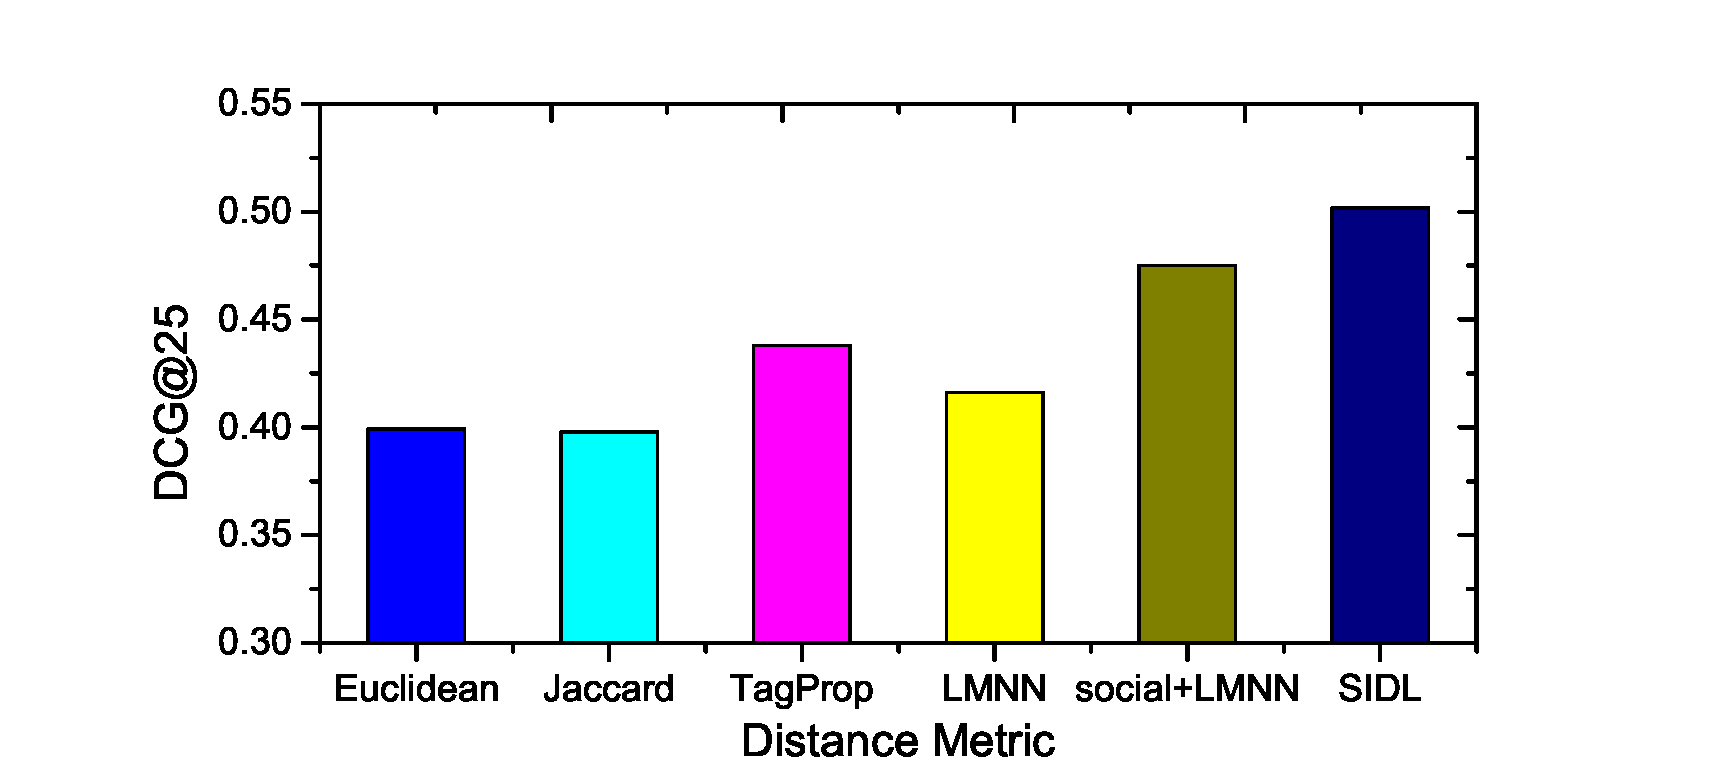
\epsfig{file=reranking.eps, width=3in}
\caption{The performance on the MSR dataset in terms of DCG@25 with using different image distance metrics in the PageRank model. }
\label{reranking}
\vspace{-0.3cm}\end{figure}
From Figure \ref{reranking}, we can observe that the Euclidean distance performs well in $DCG@25$, which is different with the previous results. It is mainly because for a given query, most of the images are visually similar. The visual words occurred are relatively concentrated. In this case, the Euclidean distance can measure the image similarity more accurate than the general images. Similar to the first experiment, \emph{TagProp} performs worse than \emph{LMNN}, which may be also caused by imbalanced training data. Based on the unsupervised PageRank model, our approach achieves $0.5017$ of $DCG@25$, which is comparable to the supervised methods reported in Multimedia Grand Challenge. It verifies the effectiveness of our approach in image reranking.

\vspace{-0.2cm}\subsection{Show Case and Insights}
In our approach, it is very interesting to observe the learned similarity from the user behavioral information. In the \emph{Mahanalobis} matrix $M$, the meaning of the $i^{th}$ diagonal element denotes the difference brought when we only add/delete the $i^{th}$ visual word in an image. Therefore, the value of the diagonal elements can be regarded as the weight of the corresponding visual words. Figure \ref{showcase1} illustrates four typical visual words with high weights in matrix $M$. Some representative images are presented at the same time. Among a huge amount of the images that include the visual word, we select the images where the visual word have similar meaning in semantic as the representative images. From Figure \ref{showcase1}, we can observe that the visual words that can represent characteristics of objects will obtain high weights in our distance learning approach, such as fruits of plants, petals, eyes of animals, branches of trees.

 Figure \ref{showcase2} reflects another interesting phenomenon.
 %In each row in Figure \ref{showcase2}, The first image and the second image are socially similar, as well as the first and the third are socially dissimilar. After learning, the visual words with high weights are labeled with red rectangles and the ones with low weights are labeled with green rectangles.
 For the three images in the first row, the first one and the second one have a common visual word on the butterfly with high weight; the first one and the third one have a common visual word on the flower with low weight. In human cognition, it is natural that the first and the second are similar because the butterfly is the focus and the flower is not very important. Here the weight of visual word can reflect this well. In the second row, three images are all about dogs. The first and the second have both eyes; the first and the third have similar furs. In emotion level, the first two images give us a feeling of ``lovely" but the third image make us fell ``lonely". Eyes of the dogs indeed play an important role in the emotion of these images, which is consistent to the weights of visual words, too. Of course, the final image distance is not determined by these several visual words. Besides, due to the semantic gap, most of visual words do not correspond to an object. Here we just try to catch a glance of the relationship between the learning results and human cognition.
\begin{figure*}\vspace{-0.3cm}
\centering
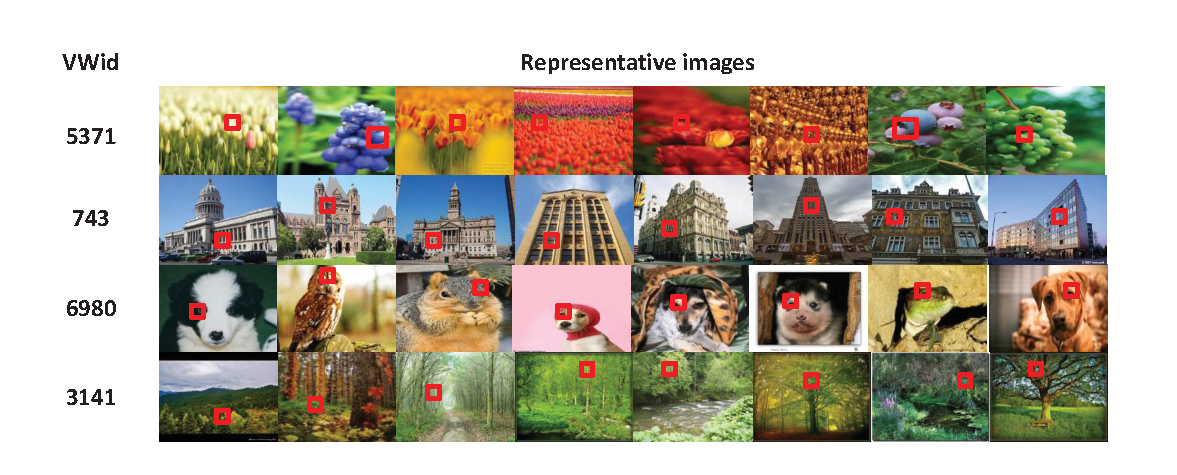
\epsfig{file=showcase_4.eps, width=6.1in, height = 2.1in}
\vspace{-0.3cm}
\caption{The illustration of the visual words with high weights in our approach. The location of the visual word is marked in a red rectangle in each image.}
\label{showcase1}
\vspace{-0.3cm}\end{figure*}
\begin{figure}
\centering
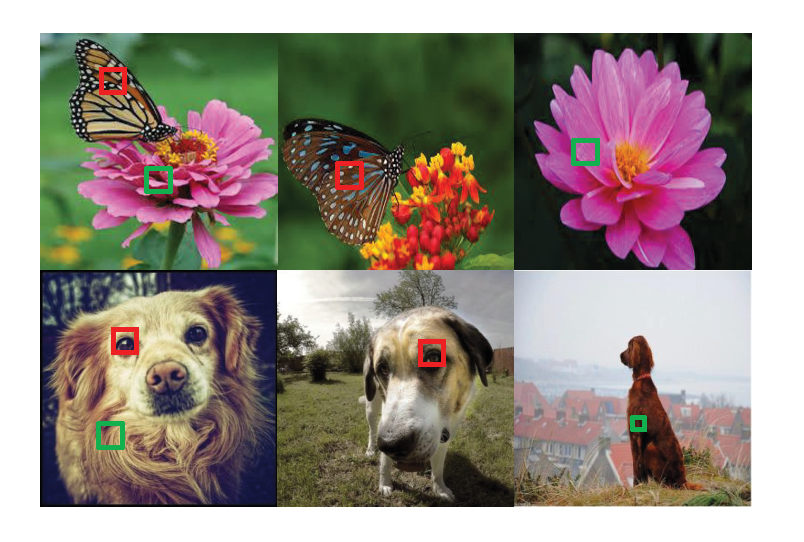
\epsfig{file=showcase_3.eps, width=3.2in, height = 1.5in}
\caption{The observations of the weight of visual words learned in our approach. In each row, The first image and the second image are socially similar, and the first and the third are socially dissimilar. Visual features with high weights are labeled with red rectangles and the ones with low weight are labeled with green rectangles.}
\label{showcase2}
\vspace{-0.3cm}\end{figure}
\vspace{-0.2cm}\section{CONCLUSION}
In this paper, we tackled evaluating image distance in the angle of human cognition for image search and recommendation. An Social embedding Image Distance Learning (\emph{SIDL}) approach was proposed to embed collective social behavioral information into visual space. \emph{SIDL} first evaluated the social similarity, where the reliability of social entities were estimated to reduce the noise and unreliability of the social data. Then a margin based metric learning algorithm was designed to learn the social similarity in visual space. In addition, we designed two application scenarios including image recommendation and image reranking where our cognitive distance can be used to reduce the cognition gap. The experiment results demonstrated that the cognitive image distance learning method was effective to learn the social similarity from BoW features. As well as the superiority of the learned image distance in image recommendation and reranking tasks had been proved.

This work is a trial to bridge the visual features and social factors to learn a ``different" cognitive image distance. Thus we only use relatively simple methods to combine the multi-dimensions of information. In the future, the power of the method can be further increased if we employ more complex features and models, for example, using deep learning on multimodal visual features.

\vspace{-0.3cm}\section{ACKNOWLEDGEMENT}
This work was supported by National Natural Science Foundation of China, No. 61370022, No.
61303075 and No. 61210008; International Science and Technology Cooperation Program of China,
No. 2013DFG12870; National Program on Key Basic Research Project, No. 2011CB302206.
 This work was also supported in part to Dr. Qi Tian by ARO grant W911NF-12-1-0057, Faculty Research Award by NEC Laboratories of America, respectively. This work was supported in part by NSFC 61128007.Thanks for the support of NExT Research Center funded by MDA, Singapore, under the research
grant, WBS:R-252-300-001-490.

\bibliographystyle{abbrv}
\small
\bibliography{sigproc}

\end{document}
